
\documentclass[11pt]{article}

\usepackage{scrextend}
\usepackage[a4paper, margin = 1.25in,footskip =0.25in]{geometry}
\usepackage{enumitem}
\usepackage{amsmath}
\usepackage{amssymb}
\usepackage{amsthm}
\usepackage{mathtools}
\usepackage{amsmath}
\usepackage{graphicx}

\newcommand{\C}{\mathbb{C}}
\newcommand{\Q}{\mathbb{Q}}
\newcommand{\R}{\mathbb{R}}
\newcommand{\Z}{\mathbb{Z}}

\graphicspath{ {images/} }

\DeclarePairedDelimiter\ceil{\lceil}{\rceil}
\DeclarePairedDelimiter\floor{\lfloor}{\rfloor}


\begin{document}
\begin{flushleft}
	Rowan Lochrin \\
	CSC445 - Alon Efrat\\
	2/15/18 \\
	Homework 2
\end{flushleft}
\begin{enumerate}
	\item Use MID5 to create characteristic hashes for every file on your
		system. MID5 is ideal for this as it's used as a checksum against
		data corruption. This means that small differences in files will result in
		large differences in hashes, so two similar files are unlikely to
		have the same hash.  We will use the characteristic hashes as
		keys for a
		hash table where the checksums are keys and the values are paths to files they
		represent. We then go through every file on the system and
		test duplicates when they collide in the table. We
		don't have to continue to probe after two entries collide in the
		table s
		when collisions happen we simply look up both files by there
		file paths.\\
		It will be necessary to generate a longer
		hash for any perspective duplicate and only report the pair if those
		hashes match. This is because the range of output of your
		hashing algorithm will be much larger then the size of the
		table.\\
		This algorithm is based on the idea that if two files are
		identical every hash of those two files will be identical. The
		core comparison stage of this algorithm, where every file is
		hashed uses a hash table so it runs in constant time per file.
		with $n$ files this algorithm is on the order of $O(n)$ and
		avoids most of the monotony that would have come from reading
		whole files to compare them with hashing.
	\item 
		\begin{enumerate}
			\item The hashing algorithm $h(k) = k\text{ mod }32$ where $k =
				0 \text{ mod } 8$ is week. The range of $h$ is only
				$\{0,8,16,24\}$ (values in $Z_{32}$, $0$ mod
				$8$). So there are only $4$ possible
				hashes that this function can output. E.g. If
				you attempted to use this to fill a $32$ row
				hash table you'd only every get entries on the
				0th, 8th, 16th, and 24th row. This will result in a
				slow table.
			\item Same thing as above, noting that $k = 0 \text{ mod
				} 32$ implies  $Ak = 0 \text{ mod } 32$.
				So the same problem applies.
			\item No, the multiplication method described in class
				involved hashing by taking the module mod $2^n
				-1$ not $2^n$. The flaw in the previous methods
				arises because $gcd(kA,m) = gcd(8,32) = 8$, so we
				restrict our range by a factor of $8$. We can see
				that $gcd(kA,m) = gcd(8,31) = 1$, meaning that
				all integers from $0,31$ are in the range of
				the function.
			\item No. To see why, consider $A \approx 7/8$. We can
				see that $Ak \mod 8 = 7$ (provided $k \neq 0$). And because
				$\gcd(7,32) = 1$ that $A$ will give us anything in the
				range. In general, we want to choose values for
				$A$ such that $\gcd(Ak \mod 8,m) = 1$. The
				downside of this hashing algorithm is that
				because of the approximate nature of floating
				point numbers we may not get the same hash every
				time. It's difficult to say how often this will
				happen but it could be massively problematic if
				it does.
		\end{enumerate}
	\item Let $\{k_1,k_2,k_3,k_4\} = \{77,147,217,287\}$.\\
		We can see that $k_1=k_2=k_3=k_4= 7 \mod 10$.
		And
		$$k_1 + i(x \mod 10) \mod m = 77 + 0 \mod 21 = 14$$
		So the first key will be inserted into index $14$.
		$$ 147 + 0 \mod 21 = 0$$
		The second key will be inserted into index $0$.
		$$ 217 + 0 \mod 21 = 7$$
		The third key will be inserted into index $7$.
		However we can see that 
		$$ 287 + 0 \mod 21 = 14$$
		Which is full so we try $i = 1$
		$$ 287 + 1(287 \mod 10) \mod 21 = 287 + 7 \mod 21 = 0$$
		Which is also full so try $ i = 2 $
		$$ 287 + 2(287 \mod 10) \mod 21 = 287 + 14 \mod 21 = 7$$
		Again full trying $i = 3$
		$$ 287 + 3(287 \mod 10) \mod 21 = 287 + 21 \mod 21  = 287 + 0
		\mod 21 = 14$$
		We can see that we will continue in this way forever, and the
		insertion fails.
	\item To do this I would give every node an attribute that can be used
		to count the number of nodes between it and the next node on the
		current level (keeping in mind nodes on lower levels). We will
		initialize this value to zero and will have to maintain this 
		counter on insertion and deletion.
		\begin{description}
			\item{\textbf{Insertion}} Every time we use the down pointer on a node we
			must increment the counter value. This is because if we
			go down the structure, we know that the node we're
			inserting is less then the next node on the
			current level. That is to say it will end up
			somewhere between them.	If we only have to insert the node at the lowest level of the
			structure this is the only change we need to make
			here.\\
			However if we are inserting a node that will need to be
			promoted to higher levels me must keep a list of all 
				the nodes that we took the down pointer on
				and a list of the number of total
				nodes we passed till we get to the next down
				pointer (or to the location of our
				insertion for the base level). For levels above
				the base
				we can accomplish this without going to the base of
				the structure by simply counting the nodes we pass
				on the current level along with the sum of the
				number of nodes in between them.
			We will call the number of total nodes we passed on level $n$ to get
				to the next down pointer $d_n$.
				In this way we can see that the number of nodes
				between our final insertion and the last node 
				before the insertion, on level $n$, for a
				skiplist of height $m$ will be
				$$d_n + d_{n+1}+...+d_m$$
				or the sum of the number of nodes we
				passed on every lower level.
			Let $v_n$ be the current value of the counter 
				on the last node on level $n$ before the
				insertion.
			Because we split the distance between the next node on
				the level when we are inserting we must subtract
				$d_n + d_{n+1} ...+ d_m$ from $v_m$ to get the
				distance between the 
				insertion node on that level and the next node
				on that level.
				We must also modify the counter to the left of
				the node by changing it to $d_n + d_n+1 + ...+
				d_m$ (or the total distance traveled before the
				insertion after we hit that node).
		A $4$ level insert is illustrated below with the counter on
				every node drawn in it's top left corners. 
		\begin{center}
		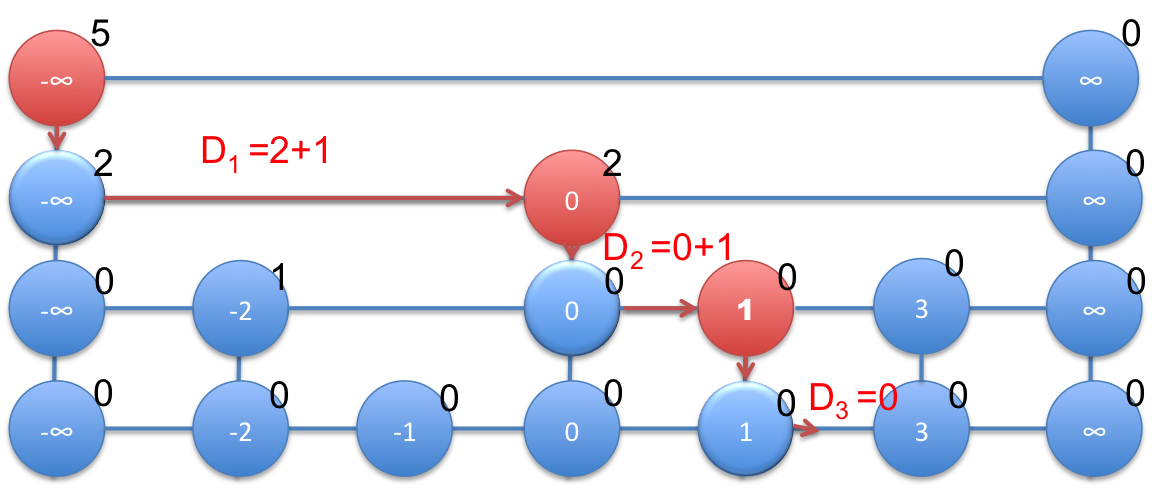
\includegraphics[width=0.85\textwidth]{images/sl1}
		\end{center}
		\begin{center}
		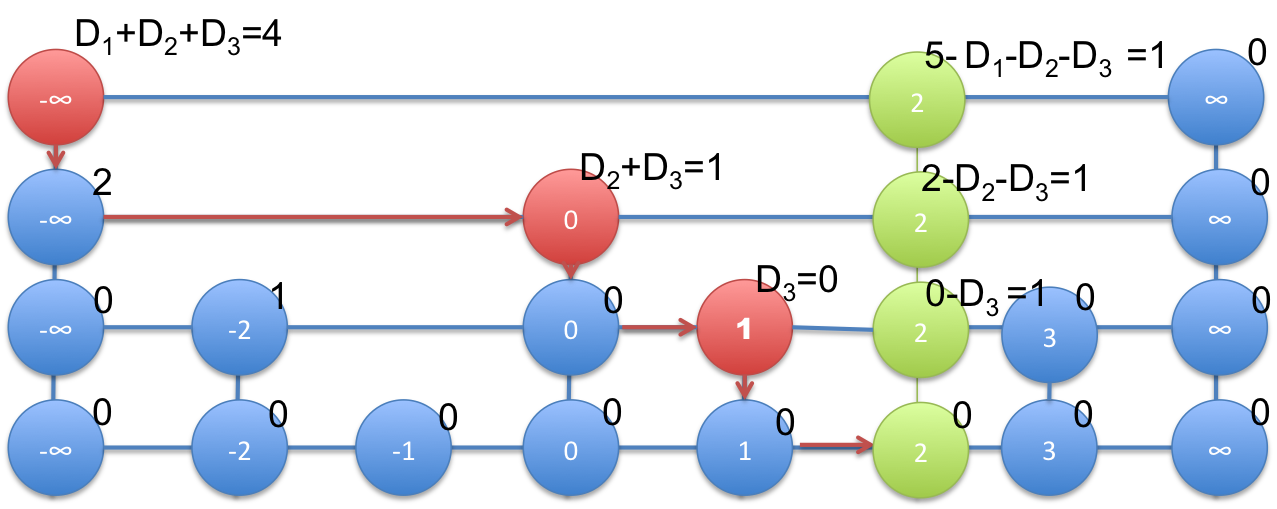
\includegraphics[width=0.85\textwidth]{images/sl2}
		\end{center}

		\item{\textbf{Deletion}}
			Deletion works in much the same way when we are deleting
				an element on the base layer, except that by
			decrementing every node we took the left pointer on
				instead of incrementing it.
			Deleting a multi-level entry can be done by adding it's
				counter on every level to the previous node
				before removing the node. This works because the
				number of nodes between the previous node and
				the new node it points to (that is the node past
				the deleted node) must be increased by the
				number of nodes between the deleted node and
				node it pointed to.
		\item{\textbf{LesserThen}}
			To create the operation we can modify the find function
				to count how many total nodes
				we pass on the way to the node we are trying to
				find. This is done by counting the nodes on every level and
				adding the number of nodes in between them. This
				will be the return value of our function.
		\end{description}
		Note that none of these changes impact the manner in which we
		traverse the tree, so insert and delete still run on
		$O(\log(n))$.
		Because LesserThen is a modification of the find function and
		also doesn't impact traversal, we know it will also run on the
		order of $O(\log(n))$.
	\item 

	\begin{enumerate}
		\item 
		The expected time for $\textit{find}(x)$ will decrease when
		$p=0.01$. To see why, consider a skiplist with $n$ elements on
		the base level. If $p = \frac{1}{2}$ then there will be an
		\begin{itemize}
		\item An average of $\frac{n}{2}$ elements on the first level.
		\item $\frac{n}{4}$ elements on the second level.
		\item $\frac{n}{8}$ elements on the third level.
		\item ....
		\item $2$ element on the $h - 1 $ level.
		\item $1$ element on the $h =\log_2(n)$ level.
			Call the element on level $h$, $P$ (for pivot).
			We will first ask the question: How many elements are
				there on level $h-1$ less $p$?
				Because there are $2$ elements on
				$h-1$ (on average) one will
				be less then $p$ and one element will be greater
				then $p$. So we only need to make one move on
				level $h$.
				Now we can consider every element less then $p$
				and every element greater then $p$
				as a skiplists of height $h-1$, and by induction
				conclude that we will have will on average 
				to make one move per level.
			So the total number of moves will be
				$$\sum_1^{\log_2(n)}2 = \log_2(n)$$
			
		\end{itemize}
		If $p = 0.01$ 
		\begin{itemize}
		\item An average of $\frac{n}{100}$ elements on the first level.
		\item $\frac{n}{100^2}$ elements on the second level.
		\item $\frac{n}{100^3}$ elements on the third level.
		\item ....
		\item $100$ elements on the $h -1$ level.
		\item $1$ element on the $h = \log_{100}(n)$ level.
		\end{itemize}
			To analyze the runtime
			of \textit{find} we note that there will be an average
			of $50$ to the left and right of $P$ meaning that the
			average number of nodes we need to touch on this level
			is $25$ as earlier we can conclude by induction that we
			will need to touch an average of $25$ nodes on every
			level. So the total number of moves will be.
				$$\sum_1^{\log_{100}(n)}25 = 25\log_{100}(n) $$
			And 
			$$25\log_{100}(n) = \frac{25 \log_2(n)}{\log_{100}(2)}
			\approx 3.76\log_2(n)$$
			So on average when $P = 0.01$ the search takes $3.76$
			times as long as it normally would.
		\item We can generalize the formula we found by noting that every level of
			our skiplist partitions the level below it into $d/n$
			partitions of size $d$. Meaning we only have to do on
			average $d/2$ comparisons on every level. 
			From here we have to figure out the height of our list
			by consider that there will be $1/d$ times the keys in
			the base level in the first level, $1/d$ times the keys
			in the second level in the first level so $1/d^2$ keys
			on. So on the $m$th level there will be $1/d^m$ keys.
			We know there will only be $1$ key on the last level so
			the height of our tree is $h$ is
			$$\frac{n}{d^h} = 1 \rightarrow n = d^h \rightarrow h = \log_d(n)$$
			So because we will have to do $d/2$ comparisons on every
			level we can write our formula for the runtime of
			\textit{find}$(x)$ as 
			$$\sum_1^{\log_d(n)}\frac{d}{2}= \frac{d\log_d(n)}{2}$$
			Graphing our function we see
		\begin{center}
		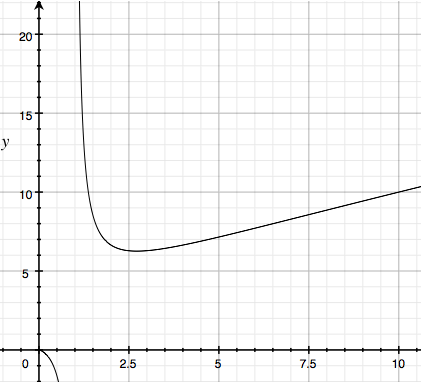
\includegraphics[width=0.75\textwidth]{images/fig3}
		\end{center}
			It has a minimum at $e \approx 2.71$.
		
	\end{enumerate}
	\item For every key is on level 1 there is a $1/2$ probability that any key will be not
		promoted to the level above it. Call key
		$k$. The probability of all $n$ keys
		not being promoted to the second level is the product
		of the individual probabilities 
		$$\prod_1^n \frac{1}{2} =\frac{1}{2^n}$$
	\item Note that whenever the top level of a skip list is empty, it is
		deleted and that the height of any particular insertion is not
		dependent on the number of nodes in the tree.
		So after removing $2^n - n$ nodes we can expect the height of
		the skip list to be the same as it would have been if we had not
		made the inserts in the first place. This means that we can use
		the formula from class and say, the probability that the skiplist is
		over height $Z\log_2(n)$ is $1/n^{Z-1}$.
	\item For $L$ our prioritized list of names, let 
		$$L = [f_1, f_2, ... ,f_n]$$
		We will use a hash table with open addressing to solve this.
		For our purposes the keys will be the names on the list and the
		values will be their respective indices (e.g. $0$ for the
		highest priority on the list). That is to say every
		name $f_i$ will be hashed to an index of the table and the value stored
		at that index will be the priority, $i$, of that name.
		Then when given two names $a,b$ we simply look them up in the
		hash table and choose the one that returns the higher priority.\\
		Inserting every name into a hash table takes $n$ time (constant time for
		every name) and searching the table runs in constant time. So
		creating a table for all $n$ males takes will take $n^2$ time.
		The next goal is to figure out how many times every individual
		table is quarried. If hypothetically every female had the same
		exact priorities list, then on every round all but one
		female would be rejected and they would all move down to their
		next choice on the list. In this way on the first round there
		are $n$ meetings, on the second round there are $n-1$ meetings
		and so on until there are no unmatched females. In this way we
		can see that there will be $n+n-1+...+1 = n(n+1)/2$ meetings and
		therefore $n(n+1)/2$ total constant time look ups so the runtime
		of our algorithm is on the order of O($n^2$).
	\item		
		\begin{enumerate}
		\item Let $p(x)$ be the preference list for a
			male or female $x$. We can see we only have to
			define
			\begin{align*}
				p(f_1) &= \{ m_1, ... \} \\
				p(f_2) &= \{ m_2, ... \} \\
				... \\
				p(f_n) &= \{ m_n, ... \} \\
			\end{align*}
			And
			\begin{align*}
				p(m_1) &= \{ f_1, ... \} \\
				p(m_2) &= \{ f_2, ... \} \\
				... \\
				p(m_n) &= \{ f_n, ... \} \\
			\end{align*}
		And we can see that everyone will go to their first
			preference on the first round, meaning no female
			will reject any male and all will be one string.
			So the algorithm terminates after one round with
			the set of pairings
			$$\{(f_1,m_1),(f_2,m_2),...,(f_3,m_3)\}$$
		\item The preferences
			\begin{align*}
				p(f_1) &= \{ m_n, ... \} \\
				p(f_2) &= \{ m_{n-1}, ... \} \\
				... \\
				p(f_n) &= \{ m_1, ... \} \\
			\end{align*}
			And
			\begin{align*}
				p(m_1) &= \{ f_n, ... \} \\
				p(m_2) &= \{ f_{n-1}, ... \} \\
				... \\
				p(m_n) &= \{ f_1, ... \} \\
			\end{align*}
			Will produce the set of pairings
				$$\{(f_1,m_n),(f_2,m_{n-1}),...,(f_n,m_1)\}$$
		\end{enumerate}
	\item First we will make an observation about the problem
		$$\Delta(p1, p2, p3) = d(p_1,p_2) + d(p_2,p_3) + d(p_3,p_1)$$
		and 
		$$d(p_2,p_3) = \sqrt{d(p_1,p_2)^2 + d(p_1,p_3)^2}  $$
		So
		$$\Delta(p1, p2, p3) = d(p_1,p_2) + d(p_1,p_3) +
		\sqrt{d(p_1,p_2)^2 + d(p_1,p_3)^2} $$
		We can minimize this function by minimizing 
		$d(p_1,p_2)^2$  and $ d(p_1,p_3)^2 $.
		So for every point, the minimum triangle connected to the point
		can be determined by finding the closest two points. Thus the
		minimum perimieter triangle can be found by going through every
		point calculating it's minimum triangle, remembering the size and
		location of the current smallest one as you go.\\
		Now we can begin our description of the algortihm. The main
		problem we hope to solve is to find the two nearest neighbors of
		any point in expected constant time. To do this we will use the
		randomized method of finding the closest pair of points approach discussed in class.  This involves taking random permutations of points and partitioning by the smallest
		distance between random pairs. The only modification we need to make to this
		algortihm is that, when visiting each point, instead of remembering the
		current closest two sets of points we need to remember both
		the perimieter of the current mimimum triangle, and the points it
		contains. At the end we will report the points it contains.
		Because the expected runtime of the original algorithm is linear and the
		only modifications we are making to it is finding $2$
		closest points for every point, and doing a slightly more
		complicated arithmatic calculation, we know that this runtime
		will also be linear.

	\item 
		Let $M_i$,$x_i$ denote the values of $M$ and $x$ on step $i$
		\begin{enumerate}
		\item
			Because $x_1 > 0$, $M_0= - \infty $ so
			$x_0 > M_0$ x $M$'s value changes. 
		\item   because $M$ changed last step we know that $M_1 = x_0$.
			And if $x_2 > M_1 $ the value of $M$ changes.
			So if 
				$\max(M_1, x_2) = \max(x_1,x_2) = x_2$	
			then $M$'s value changes. Since both our random
			variables are in the same range the chance of this will be $1/2$
		\item From the earlier step we know $M_2 = \max(x_1,x_2)$ and
			$M$ will change if
			$$M_3 = \max(M_2,x_3) = \max(\max(x_1,x_2),x_3)
			= \max(x_1,x_2,x_3) = x_3$$
			And the probablity of that happening is $1/3$.
		\item Because count is incremented on every successful change of
			$M$ and we can see from the earlier step that the odds
				of that happening are $1/m$ on step $m$, we can
				see for steps one thorugh $n$ that the average amount
				the count changes is
			$$ \frac{1}{2}+ \frac{1}{3}+ \frac{1}{4} +...+
				\frac{1}{n} = \sum_{i = 1} ^ n \frac{1}{i}
				\approx 0.577 \log(n) $$

		\end{enumerate}
	\item Assuming the unrandomized approach.
		\begin{enumerate}
		\item We first insert two points in the hash table $p_1,p_2$ and calculate
			the distance between them, then partition the space
				into a grid of size $d(p_1,p_2)/2$, add a third point $p_3$ and
			partition around it to determine if there is a point
				closer then the current mimimum distance
				$d(p_1,p_2)$. Because every square has
				size $d(p_1,p_2)/2$ this means that any partition
				with any point closer to $p_3$ than $p_1$ is
				to $p_2$ will be under two partitions away from
				the parition containting 
				$p_3$. Meaning we only have to check the $5x5$
				grid centered around the partition $p_3$ contains,
				or $25$ partitions  total. 
				This is illustrated below with the checked partion in
				gray. Note that we check all corners as
				calculating weather or not to include them would
				probably cost about as much computation.\\
				Because we have to do this for all points except
				$p_1,p_2$ we will have to make $25(n-2)$
				lookups.
				
		\begin{center}
		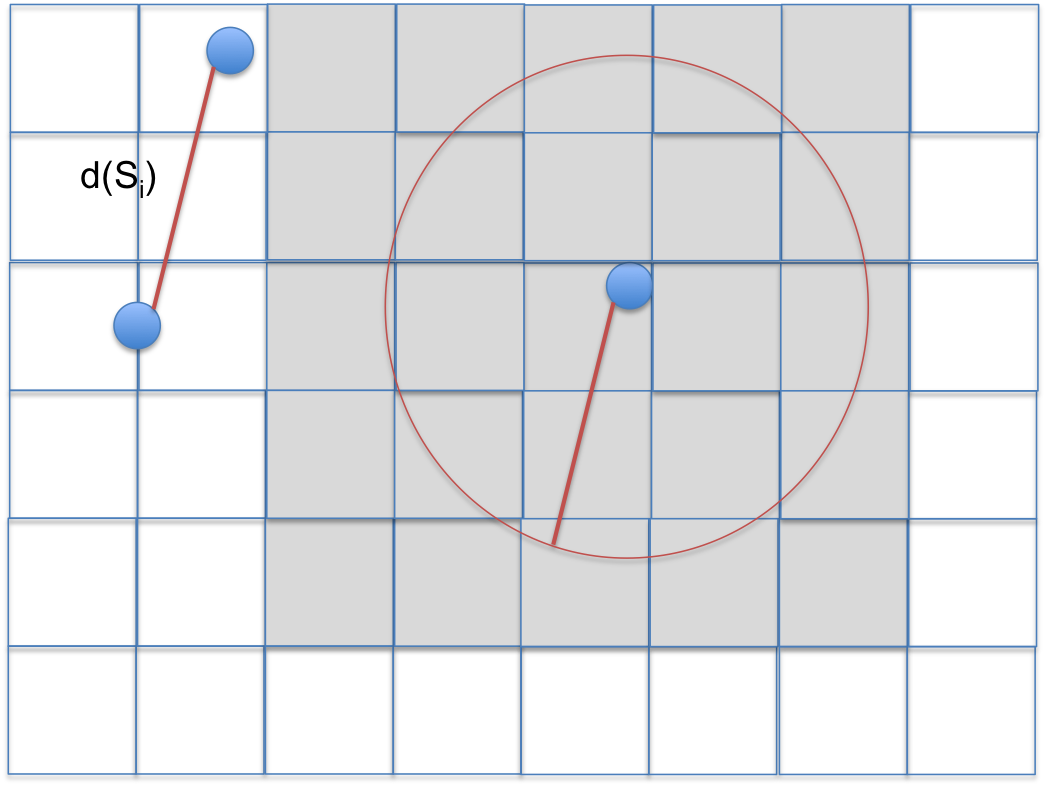
\includegraphics[width=0.65\textwidth]{images/fig4}
		\end{center}
		\item Doing this in one dimension, the only modification we have to
			make is to consider that the radius of two partitions around the
			partition containing the insertion point will simply be the
				line containing $5^1$ partitions.
		\item In three dimensions we must look at the cube containg $5^3
			= 125$ partitions around the point. In general, in $n$
				dimensions we must look at the $5^n$ partitions
				around the insertion partitions.
		\end{enumerate}
\end{enumerate}
\end{document}

